% diagram.tex - DESC
% Iago Mosqueira - JRC. 2013
%
\documentclass[tikz]{standalone}
\usepackage{tikz,amsmath}
\tikzstyle{end} = [circle, minimum width=3pt, fill, inner sep=0pt, right]
\begin{document}
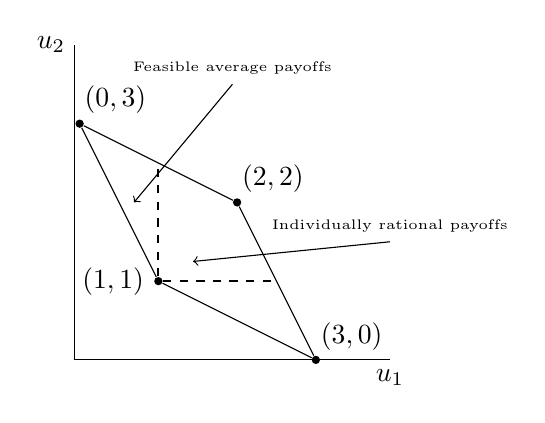
\begin{tikzpicture}
    \draw (0,0) -- (4,0) node [below] {$u_1$};
    \draw (0,0) -- (0,4) node [left] {$u_2$};
    \draw (3,0) node[end] (A) {} node [above=.3cm,right] {$(3,0)$};
    \draw (0,3) node[end] (B) {} node [above=.3cm,right] {$(0,3)$};
    \draw (1,1) node[end] (C) {} node [below,left] {$(1,1)$};
    \draw (2,2) node[end] (D) {} node [above=.3cm,right] {$(2,2)$};
    \draw (A) -- (D);
    \draw (D) -- (B);
    \draw (B) -- (C);
    \draw (C) -- (A);
    \draw [dashed,thick] (C) -- ++(0,1.5);
    \draw [dashed,thick] (C) -- ++(1.5,0);
    \draw [->] (2,3.5) node[above] {\tiny{Feasible average payoffs}} -- (.75,2);
    \draw [->] (4,1.5) node[above] {\tiny{Individually rational payoffs}} -- (1.5,1.25);
\end{tikzpicture}
\end{document}
